\chapter{Extension Complexity}

\section{LPs \& Its Two Views}
Extension Complexity pertains how much power lies within linear programs. First, we state the canonical form of Linear Programs (LP). 
\begin{definition}
	[Linear Program]
	A linear program take the following vectorized canonical form
	\begin{align}
		\text{maximize} &\quad \quad  \bc^\top \bx \\
		\text{subject to} & \quad \quad A\bx \leq \bb 
	\end{align}
\end{definition}

We here illustrate the two views of Linear Programs. First, we consider the dimension to optimize over is $n = 2$. Then, if we unwrap the vectorization we have the constraints
\begin{equation}
	\begin{bmatrix}
		a_1^1x_1 + a_2^1 x_2 \\
		\vdots \\
		a_1^m x_1 + a_2^m x_2
	\end{bmatrix} 
	\leq 
	\begin{bmatrix}
		b_1 \\
		\vdots \\
		b_m
	\end{bmatrix}
\end{equation}

Now, if we plot the lines corresponding to the linear constraints, we will get something like Figure \ref{fig:lp-view}. Considering the fact that we are optimizing over a linear objective, the maximizer must appear on the vertices of the formed polytope. We call the region bounded in between all the constraints the feasible region of the Linear Program and each edge segments as ``facets''. Two views arise in this formulation. 

\begin{figure}
	\center
	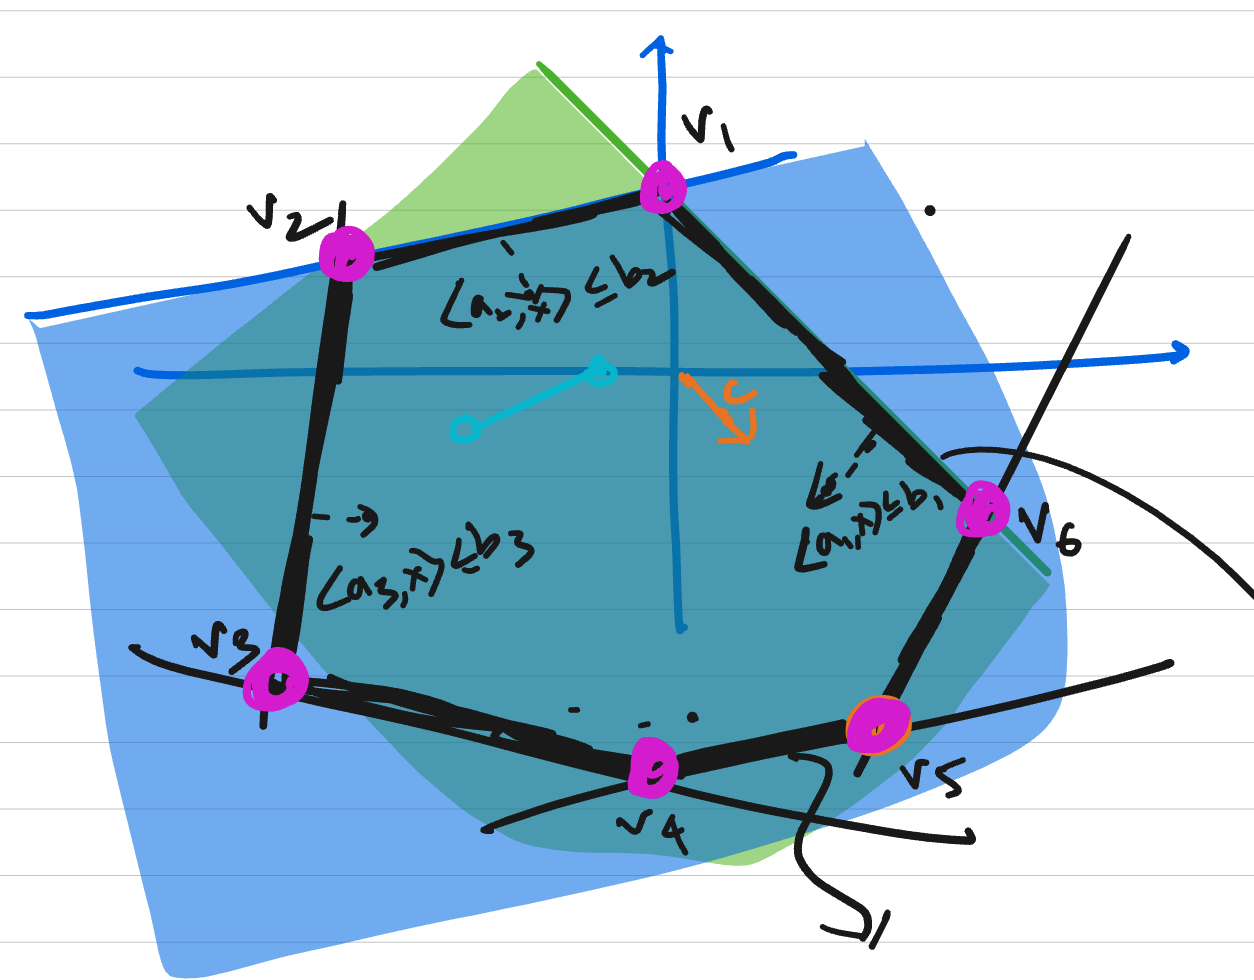
\includegraphics[width=0.6\textwidth]{figs/lp-view.png}
	\caption{Plotted LP constraints}
	\label{fig:lp-view}
\end{figure}

\paragraph{Polyhedron View} says that the feasible region is the \textbf{\textit{intersection}} of the linear inequalities. Notice that we are strictly limiting ourselves to the intersections here, no area included. 

\paragraph{Polytope View} says that the feasible region can be stated as 
\begin{equation}
	Convex-Hull \{ v_1, \dots v_6 \}
\end{equation}

where we define 
\begin{definition}
	[Convex Hull]
	Given $S = \{v_1, \dots, v_N \}$, then
	\begin{equation}
		Convex-Hull(S) = \left\{ x: x = \sum_i \lambda_i v_i, \quad \quad s.t. \quad \lambda_i \geq 0, \sum_i \lambda_i = 1 \right\}
	\end{equation}
	Remark: The formed set is convex, since for all $x, y \in S$, so does $(x + y) / 2 \in S$. 
\end{definition}

Now that we defined the two formulations, we state the equivalence. 
\begin{equation}
	\left.\begin{aligned}
		\max \langle \bc, \bx \rangle \\
		x_i \in \{0, 1\}^n \\
		\sum x_i \leq n / 2
	\end{aligned} \right\}
	\quad \quad \equiv \quad \quad \left\{
	\begin{aligned}
		\max \langle \bc, \bx \rangle \\
		0 \leq x_i \leq 1 \\
		\sum x_i \leq n / 2
	\end{aligned} \right.
\end{equation}
With this equivalent, we have only $2n + 1$ facets to optimize over, and hence we can solve it efficiently. 


\section{Extension Complexity and Cross Polytope}
The Cross Polytope example will help us find and define the extension complexity ``gap''. We start with the definition

\begin{definition}
	[Cross Polytope]
	\begin{equation}
		Cross-Polytope \equiv Convex-Hull \{ e_1, -e_1, e_2, -e_2, \dots, e_n, -e_n \}
	\end{equation}
	where $e_i \in \{0, 1\}^n$ is the standard indicator vector.
\end{definition}

Notice that here we essentially have a hypercube, in $n$ dimensions, meaning it needs $2^n$ inequalities to specify. But also, from the definition, we see there are only $2n$ vertices. Hence, there is a big gap between number of vertices and number of inequalities is. 

We now take a look at the cross polytope in an alternative view
\begin{align}
	Cross-Polytope 
	&= \left\{ \bx : \sum_{i = 1}^n |x_i| \leq 1 \right\} \\
	&= \left\{ \bx : \exists \by, \quad s.t. \quad
		\sum y_i \leq 1 \,\,\wedge\,\,
		-y_i \leq x_i \leq y_i \right\}
\end{align}

where notice that by adding a new variable $\by$, we are able to describe cross-polytope with only $2n + 1$ inequalities. We define this gap as the extension complexity. Formally, 

\begin{definition}
	[Extension Complexity (Yannakaskis, 88)]
	The extension complexity of a convex polytope $P$ is the smallest number of facets among convex polytopes $Q$ that have $P$ as a projection. In this context, $Q$ is called an extended formulation of $P$; and it may have much higher dimension than $P$. 
	
	In English: we are given the freedom to add variables. Now, with this power, we want to minimize the number of inequalities. What is the minimum number of inequalities needed to describe the initial problem in this setting? 
	
	We denote extension complexity as $XC(P)$ = minimum number of facets of $Q$ over all extensions $Q$ of $P$. 
\end{definition}

Following the notation appeared in the definition, we consider $P$ a polytope
\begin{equation}
	P = Convex-Hull \{ v_1, \dots, v_n \}
\end{equation}
and $Q \subseteq \real^{n + m}$ is an extension of $P$ if 
\begin{equation}
	P = \{ \bx : \exists \by, (\bx, \by) \in Q \}
\end{equation} 

To rephrase from the definition, the idea here is that there are many possible extensions ($Q$). Maybe some $Q$ can be defined with fewer inequalities and define $XC(P)$ as the minimum number of inequalities needed across all extensions. 

Notice that the extended form can easily be written down as a equivalent form of the original optimization goal 
\begin{equation}
	\begin{aligned}
		\max \langle \bc, \bx \rangle \\
		\bx \in P
	\end{aligned}
	\quad \quad
	\equiv 
	\quad \quad 
	\begin{aligned}
		\max \langle (\bc, 0), (\bx, \by) \rangle \\
		(\bx, \by) \in Q
	\end{aligned}
\end{equation}

Recall at the cross polytope example we presented at the beginning of this section. We have shown the upper bound 
\begin{equation}
	XC(Cross-Polytope) \leq 2n + 1
\end{equation}

\section{Examples}
\subsection{Permutahedron}
We start by defining a permutahedron. 
\begin{definition}
	[Permutahedron]
	As the name suggests, a permutahedron is formed by vertices such that they are permutations of each other. 
	\begin{equation}
		\real^n \supseteq P_n = Cvx \{ (1, 2, 3, \dots, n) , (2, 1, 3, \dots, n) , \dots  \}
	\end{equation}
	which is a convex hull formed by $n!$ vertices. 
\end{definition}
For a permutahedron, we find that
\begin{proposition}
	[Facets and Vertices of Permutahedron] 
	\begin{equation}
		\# vertices (P_n) = n! \quad \quad \# facets (P_n) = 2^n
	\end{equation}
\end{proposition}

Now, suppose we wish to optimize over this permutahedron set $P_n$, we have 
\begin{equation}
	\begin{aligned}
		\max \quad \langle \bc, \bx \rangle \\ 
		\langle \ba_1, \bx \rangle \\
		\vdots \quad \\
		\langle \ba_N, \bx \rangle \\
		\text{where } x \in P_n
	\end{aligned}
\end{equation}

\begin{proposition}
	[Bounds on Permutahedron]
	Birkoff-Von Neuman Theorem states that 
	\begin{equation}
		XC(P_n) \leq n ^2
	\end{equation}
	and this is later improved by Goemans to 
	\begin{equation}
		XC(P_n) \leq \mathcal O (n \log n)
	\end{equation}
\end{proposition}

\subsection{Spanning Tree Polytope}
\begin{definition}
	The spanning tree polytope is defined as follows
	\begin{equation}
		\real^{C^n_2} \supseteq SP_n = Cvx (\text{indicator vectors of spanning tree})
	\end{equation}
\end{definition}
The definition above seem rather abstract. Here is an example. Consider a graph with four nodes. Then, there are at most $C^n_2 = C^4_2 = 6$ edges in this graph, and then we can represent the edges with indicators. I.e., we have possible edges
\begin{equation}
	(a, b) \quad (a, c) \quad (a, d) \quad (b, c) \quad (b, d) \quad (c, d)
\end{equation}
and it suffices to use indicators to denote which edges are chosen. 

For example, consider the following graph which looks like a chain
\begin{equation}
	a - b - c - d 
\end{equation}
it takes indicator form 
\begin{equation}
	(1, 0, 0, 1, 0, 1)
\end{equation}
we verify that a three edged graph has three 1's in its corresponding indicator vector. 

Handling weighted graph is simple, we only need to replace all the 0's with $\infty$'s to signify that choosing them incurs infinity penalty; we also replace the 1's with respective weights of the edges. 

In the classic Minimum Spanning Tree (MST) problem, we aim to find a set of edges in a graph such that it forms a tree and has the lowest total weight. This problem can be translated into LP with the help of our indicator formulation, 
\begin{equation}
	MST \quad \equiv \quad \begin{aligned}
		\min \, \langle \bw_G, \bx \rangle \\
		\bx \in SP_n
	\end{aligned} \quad \equiv - \begin{pmatrix}
		\max \, - \langle \bw_G, \bx \rangle \\
		\bx \in SP_n
	\end{pmatrix}
\end{equation}

\begin{proposition}
	[Vertices and Facets in Spanning Tree Polytope] 
	\begin{align}
		\# vertices (SP_n) = \# trees \quad \quad \# facets (SP_n) = 2^n
	\end{align}
\end{proposition}

\begin{proposition}
	[Extension Complexity of Spanning Tree Polytope]
	\begin{equation}
		XC(SP_n) = \mathcal O( n^3 )
	\end{equation}
\end{proposition}

\subsection{TSP Polytope}
\begin{definition}
	[TSP Problem]
	Given a weighted graph, $G = (V, E)$, find the tour of a least total weight; where tour is defined as a loop inside the graph that visits every vertex exactly once, finishing at the starting position. 
\end{definition}

\begin{definition}
	[TSP Polytope]
	\begin{equation}
		\real^{C^n_2} \supseteq Cvx (\text{all valid tours encoded with indicator vectors})
	\end{equation}
	where the definition utilizes the indicator trick for specifying graphs we say in the previous spanning tree polytope example. 
	
	With this definition, our TSP problem turns into the following optimization problem 
	\begin{equation}
		\begin{pmatrix}
			\min \, \langle W_G, \bx \rangle \\ 
			\bx \in TSP_n
		\end{pmatrix}
		\quad 
		\equiv \quad
		\text{find minimum tour of $G$}
	\end{equation}
\end{definition}

\begin{proposition}
	[Vertices and Facets of TSP Polytope]
	\begin{equation}
		\# vertices (TSP_n) = n! \quad \quad \# facets (TSP_n) = 2^n
	\end{equation}
\end{proposition}
 
In the previous examples, we were lucky to find polynomial extension complexities. However, for TSP, a known NP-Complete problem, we are not so lucky. The question then to ask is what is $XC(TSP_n)$? 

\begin{theorem}
	[Y88, Symmetric Extension Complexity]
	\begin{equation}
		XC_{Symm} (TSP_n) \geq 2^{\Omega(n)}
	\end{equation}
	i.e., is at least exponential. If we restrict the $TSP_n$ such that the graphs inside are symmetric, then we cannot get much savings. 
\end{theorem}

The remaining question to ask is what is $XC(TSP_n)$? This was left as an open question in the original paper. 

\section{FMPTW12 \& Alternative Proof}
\subsection{Non-Negative Rank and Extension Complexity}
\begin{theorem}
	[Fiorini, Massor, Prokutta, Tiwary, Wolf (FMPTW12)]
	\begin{equation}
		XC(TSP_n) \geq 2 ^{\Omega (n)}
	\end{equation}
	\label{thm:FMPTW12}
\end{theorem}

\begin{definition}
	[Slack Matrix]
	Consider the polytope, written in the forms both as a convex hull and as a polyhedron
	\begin{equation}
		P = Cvx\left( \bx_1, \dots, \bx_N \right) = \{\bx: \langle a_j , \bx \rangle \leq b_j\,, j = 1, \dots, N \} 
	\end{equation}
	Whenever we have the above, Slack Matrix $S \in \real^{N \times M}$ can then be defined as 
	\begin{equation}
		S[i,j] = b_j - \langle a_j , x_i \rangle
	\end{equation}
	i.e. ``how much slack is there in the $j$-th inequality for vertex $i$. 
	
	\paragraph{Non- negative Property} We note that the slack matrix has entries $S[i, j] \geq 0, \forall i, j$. 
\end{definition}

\begin{definition}
	[Rank]
	Recall from LA that the rank of a matrix $rank(S)$ is either of the following
	\begin{itemize}
		\item dimension of the space spanned by the rows of $S$, the row space
		\item dimension of the space spanned by the columns of $S$, the column space
		\item minimum $r$ such that $S$ can be written as $S = UV^\top$, where $U \in \real^{N \times r}$ and $V^\top \in \real^{r \times M}$.   
	\end{itemize}
\end{definition}

\begin{definition}
	[Non Negative Rank (NNR)]
	If we have a non negative matrix, the NNR is a similar notion. Formally, if we have matrix $S \geq 0$, then 
	\begin{equation}
		nnr(S) = \min_r \left\{
			S = U V^\top 
		\right.
	\end{equation}
	where $\real^{N \times r} \ni U \geq 0$ and $\real^{r \times M} \ni V^\top \geq 0$. Notice that here we added an additional requirement for the factorized matrices to also be non negative. 
\end{definition}

\begin{proposition}
	\begin{equation}
		rank(S) \leq nnr(S) \leq \min(N, M)
	\end{equation}
\end{proposition}

\begin{theorem}
	[NNR and XC, Y88]
	If $P$ is a polytope and $S$ is a slack matrix of $P$, then 
	\begin{equation}
		XC(P) = nnr(S)
	\end{equation}
	\label{thm:NNR and XC, Y88}
\end{theorem}
This theorem relates something geometric (XC) to a very concrete computable value. We will use this to prove Theorem \ref{thm:FMPTW12}, i.e. we try to show $nnr$ (slack matrix of $TSP_n$) = $2^{\Omega(n)}$. We will not show this exactly. Instead, we show it for another polytope, which has a reduction to $TSP_n$. We leave that to later part of this chapter. Let's show Theorem \ref{thm:NNR and XC, Y88}.
  
\begin{proof}
	We show it from two inequalities. First, we show 
	\begin{equation}
		XC(P) \leq nnr(S)
	\end{equation}
	To be exact, we want to show: if $nnr(S) = r$, then there is an extension of $P$ with $\leq r$ inequalities. From definitions, we can write
	\begin{equation}
		S = UV, \quad \quad U\geq0, V \geq 0, U \in \real^{N \times r}, V \in \real^{r \times M}
	\end{equation}
	Call the rows of $U$ as $u_i$ and the columns of $V$ as $v_j$. Then, 
	\begin{equation}
		b_j - \langle a_j, \bx_i \rangle = S[i, j] = \langle u_i, v_j \rangle
	\end{equation}
	where $i, j$ corresponds to indices of vertices and inequalities respectively. We can massage the above equality to form
	\begin{align}
		&\langle a_j, x_i \rangle + \langle u_i, v_j \rangle = b_j \\
		\iff &\langle (a_j, v_j), (x_i, u_i) \rangle = b_j 
	\end{align}
	Recall definition of $P$,
	\begin{equation}
		P = \{x: Ax \leq b \}
	\end{equation}	
	Now we define a new extension
	\begin{equation}
		Q = \left\{ (x, u) : Ax + Vu = b , u \geq 0 \right\} = \left\{ (x, u) : \langle a_j, x \rangle + \langle v_j , u \rangle = b_j , u \geq 0 \right\}
	\end{equation}
	and we claim that this $Q$ is an extension of $P$. For verification, we need to check (the definition
	\begin{equation}
		\forall x \in P, \exists n \text{ s.t. } Ax + Vu = b
	\end{equation}
	which clearly is the case. 
	
	Now, we show the other direction inequality, $nnr(S) \leq XC(P)$. Suppose we have an extension $Q$ of $P$ with few inequalities: 
	\begin{equation}
		Q = \left\{ 
			(x, y) : Ex + Fy \leq d
		\right\} 
	\end{equation}
	From definitions, if $Q$ is indeed an extension of $P$, then 
	\begin{align}
		P 
		&= \left\{
			x : \exists y, (x, y) \in Q
		\right\} \\
		&= \left\{ 
			x : \langle a_j, x \rangle \leq b_j, \quad \forall j = 1, \dots, m
		\right\} \\
		&= Cvx \{x_1, \dots, x_N \}
	\end{align}	
	The above equality of sets implies 
	\begin{align}
		&\text{if } (x, y) \in Q, \text{ then } \langle a_j, x \rangle \leq b_j \quad (\forall j) \\
		\equiv\quad &(x, y) \in Q \implies \langle (a_j, 0), (x, y) \rangle \leq b_j \quad (\forall j) \\
		\equiv\quad & Ex + Fy \leq d \implies \langle (a_j, 0), (x, y) \rangle \leq b_j \quad (\forall j)
	\end{align}
	
	We introduce the following Lemma
	\begin{lemma}
		[Strong Farkas' Lemma]
		\begin{equation}
			\left. 
				\begin{aligned}
					\langle (e_1, f_1) , (x, y) \rangle \leq d_1 \\
					\vdots \quad \quad \quad \quad \\
					\langle (e_r, f_r), (x, y) \rangle \leq d_r
				\end{aligned}
			\right\} \implies \langle g, (x, y) \rangle \leq h
		\end{equation}
		\textbf{\textit{if and only if}} $\exists u_1, \dots, u_r \geq 0, \, s.t.$
		\begin{equation}
			g = u_1 (e_1, f_1) + u_2 (e_2, f_2) + \dots u_n (e_r, f_r)
		\end{equation}
		and \begin{equation}
			h = u_1 d_1 + u_2 d_2 + \dots u_r d_r
		\end{equation}
		
		\paragraph{Matrix Form (SFL)} If $Ex + Fy \leq d \implies \langle g, (x, y) \rangle \leq h$, then $\exists u \geq 0$ such that  
		\begin{equation}
			u^\top \begin{bmatrix}
				[E] & [F]
			\end{bmatrix} = g \quad ; \quad \quad u^\top d = h
		\end{equation} 
	\end{lemma}
	
	Recap: we have 
	\begin{equation}
		Ex + Fy \leq d \implies \langle (a_j, 0) , (x, y) \rangle \leq b_j
	\end{equation}
	in particular, this implies $\exists v_j$ such that 
	\begin{equation}
		\begin{matrix}
			v_j^\top \begin{bmatrix}
				[E] & [F]
			\end{bmatrix} = a_j \\
			v_j^\top d = b_j
		\end{matrix}
	\end{equation}
	
	Define a new vector $u_i = d - Ex_i - Fy_i \in \real^r$. We claim that (1) $u_i \geq 0, v_j \geq 0$ as vectors and (2) $\langle u_i, v_j \rangle = b_j - \langle a_j, x_i \rangle = S[i, j]$. 
	
	Now, we plug in $u_i$ into the views we had previously, to find 
	\begin{equation}
		v_j ^\top \begin{bmatrix}
			[E] & [F]
		\end{bmatrix} = (a_j, 0) \quad v_j^\top d = b_j \quad u_i = d - Ex_i - Fy_i
	\end{equation} 
	Then, 
	\begin{align}
		v_j^\top u_i 
		&= \langle v_i, d \rangle - v_j^\top \begin{bmatrix}
			[E] & [F]
		\end{bmatrix} \begin{bmatrix}
			[x_j] \\ [y_j]
		\end{bmatrix} \\
		&= b_j - \langle a_j, x_i \rangle 
	\end{align}
	This implies 
	\begin{equation}
		nnr(S) \leq r = XC(P)
	\end{equation}
	Therefore, 
	\begin{equation}
		nnr(S) = XC(P)
	\end{equation}
	as wanted. \qed
\end{proof}

With this theorem, in order to study extension complexity, we only need to study non negative rank. 


\subsection{Proof with Correlation Polytope}
\begin{definition}
	[Correlation Polytope]
	A correlation polytope is
	\begin{equation}
		CP_n = Cvx \left( \left\{ aa^\top: a \in \{0, 1\}^n \right\} \right)
	\end{equation}
\end{definition}

\begin{proposition}
	We can write any graph optimization problem as a linear optimization problem on $CP_n$. 
\end{proposition}

\begin{proposition}
	\begin{equation}
		XC(CP_n) \leq XC(TSP_n) 
	\end{equation}
\end{proposition}

\begin{theorem}
	[Extension Complexity of Correlation Polytope (FMPTW12)]
	\begin{equation}
		XC(CP_n) \geq 2^{\Omega (n)}
	\end{equation}	
\end{theorem}

\begin{definition}
	[Partial Slack Matrix]
	Suppose we have polytope $P \in \real^N$. We have another polytope which has containment relationship $P \subseteq P'$, say defined as $P' \equiv \{ x: Cx \leq d \}$. Then, every vertex / point in the polytope $P$ must also satisfy the definition of $P'$.  
	
	Define 
	\begin{equation}
		Slack(P,P')[i, j] = d_j - \langle c_j , x_i \rangle \geq 0
	\end{equation}
\end{definition}

Y88 also showed that if $P \subseteq P'$, then
\begin{equation}
	XC(P) \geq nnr(Slack(P, P'))
\end{equation}
Hence, if are smart or lucky enough, we can find a $P'$ that results in a easy to study $Slack(P, P')$ partial slack matrix instead. In FMPTW12, they proposed to construct the following $P'$. For every $b \in \{0, 1\}^n$, let $C_b = 2\cdot \mathrm{diag} (b) - bb^\top $. Then, define
\begin{equation}
	P' = \left\{ x \in \real^{n \times n} : \langle C_b, x \rangle \leq 1, \quad \forall b \in \{0, 1\}^n \right\}
\end{equation}
 
\begin{proposition}
	We claim that the $P'$ composed this way is a superset of the $CP_n$ polytope that we want to study. 
	\begin{equation}
		CP_n \subseteq P'
	\end{equation}
\end{proposition}

\begin{proof}
	From definition, 
	\begin{equation}
		CP_n = Cvx ( \{ aa^\top : a \in \{0, 1\} ^n \} )
	\end{equation}
	We need to show that $\langle aa^\top , C_b \rangle \leq 1$ for all $a \in \{0, 1\} ^n $. Note that
	\begin{align}
		& \langle aa^\top, C_b \rangle \leq 1 \\
		\iff & \langle aa^\top , 2 \cdot \mathrm{diag} (b) - bb^\top \rangle \leq 1 \\
		\iff & \langle aa^\top , 2 \cdot \mathrm{diag} (b) \rangle - \langle aa^\top, bb^\top \rangle \leq 1 \\
		\iff & 2 |a \cap b | - (a^\top b ) ^2 \leq 1 \\
		\iff & 2 |a \cap b | - |a \cap b | ^2 \leq 1 \\
		\iff & 0 \leq 1 + |a \cap b|^2 - 2 |a \cap b| 
				= ( a - |a \cap b| ) ^ 2
	\end{align}
	where the notation $|a \cap b |$ denotes the number of entries where $a$ and $b$ intersect. \qed
\end{proof}

In the notation $Slack(P, P')$, 
\begin{itemize}
	\item $P$ has $2^n$ vertices corresponding to $a \in \{0, 1\}^n$, and 
	\item $P'$ has $2^n$ inequalities corresponding to $b \in \{0, 1\}^n$. 
\end{itemize}

Recall that the slack matrix is such that (1) rows are indexed by vertices and (2) columns are indexed by constraints. Hence if we allow a bit of abuse of notation, we can derive $Slack(P, P')_{a, b}$  
\begin{proposition}
	\begin{equation}
		Slack(P, P')_{a, b}  = (1 - |a \cap b |) ^ 2
	\end{equation}
\end{proposition}
\begin{proof}
	The derivation above tells us that $\langle aa^\top, C_b \rangle = (1 - |a \cap b| ) ^2$. We can use this to come up with an alternative form of the slack matrix. 
	\begin{align}
		Slack(P, P')_{a, b} 
		&= 1 - \langle C_b, aa^\top \rangle \\
		&= (1 - |a \cap b |) ^ 2 \\
		&\triangleq M
	\end{align}
	At the end of the day, the partial slack matrix for our $P. P'$ has a very simple description! This concludes the proof. \qed
\end{proof}

For the matrix $M$, define 
\begin{equation}
	D = \{ (a, b) : |a \cap b| = 0 \} \quad \quad U = \{ (a, b) : | a \cap b | = 1 \}
\end{equation}
so cells in $M$ belongs to one of these two disjoint sets, either $D$ or $U$. This is to say (1) $M_{ab} = 0$ for $(a, b) \in U$, and (2) $M_{ab} = 1$ for $(a, b) \in D$. 

Suppose $M$ has a small non-negative rank factorization, i.e 
\begin{equation}
	M = UV \quad \quad U \in \real^{2^n \times r} \geq 0, V \in \real^{r \times 2^n} \geq 0
\end{equation}
since this is a nonnegative rank factorization, we have non negative entries in $U$ and $V$. Let $U_i$ denote the $i$-th column and $V_j$ denote the $j$-th row, then entries inside $U_i$ and $V_j$ are either positive or zero. We break the matrix product into sum of their row / column outer products and look at the positive entries only (see Figure \ref{fig:nnr-inclass-positive}).   

\begin{figure}
	\center
	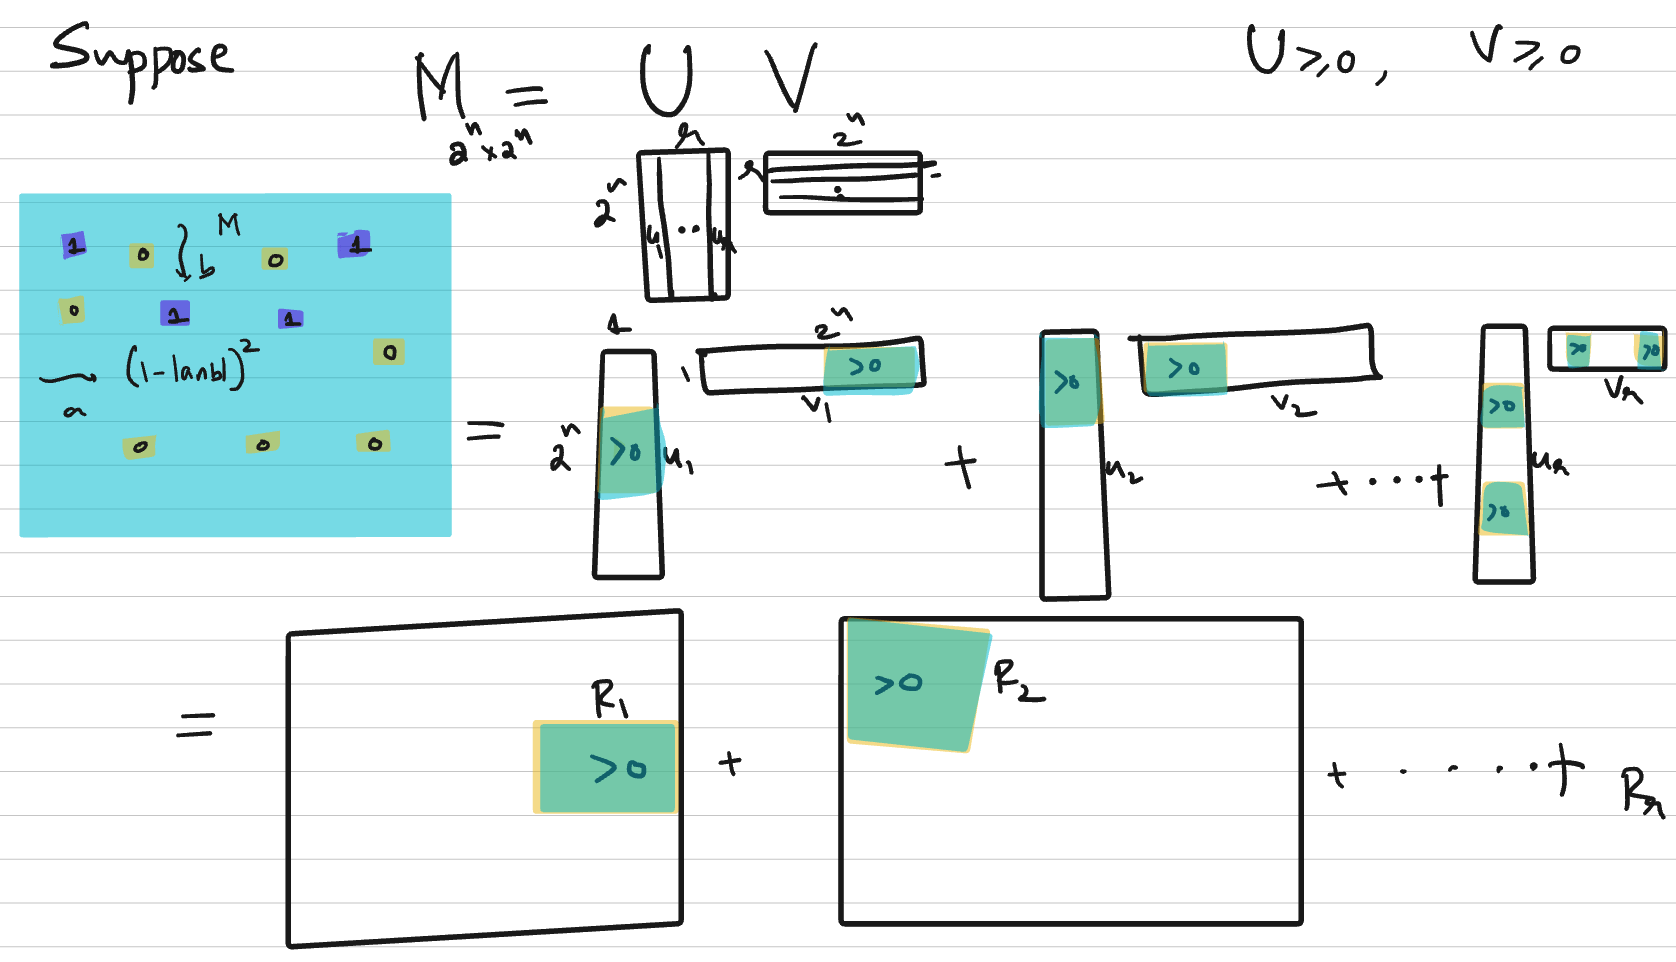
\includegraphics[width=0.8\textwidth]{figs/nnr-inclass-positive.png}
	\caption{We can break down the matrix product $UV$ into sum of outer products of their columns and rows. Due to NNMF, we only look at the positive patches in the vectors and this results in a form with addition of positive patches in the matrix. }
	\label{fig:nnr-inclass-positive}
\end{figure}
 
We define a series of ``rectangles'', which represents patches of positive entries illustrated in Figure \ref{fig:nnr-inclass-positive}. Let
\begin{equation}
	R_{i} = \left\{ 
		(a, b) : \text{$U_i$ is positive at $a$, $V_i$ is positive at $b$}
	\right\}
\end{equation}

\begin{proposition}
	[Properties of ``Rectangle'']
	The series of rectangles $R_1, R_2, \dots, R_r$ has the following magical properties
	\begin{itemize}
		\item $\bigcup_{i = 1}^r R_i$ must cover all points in $D$, and 
		\item $R_i \cap U = \emptyset$ for all $i = 1, \dots, r$
	\end{itemize}
\end{proposition}

This property is already known thanks to Razborov, where he stated
\begin{theorem}
	[Razborov's Extension on Magical Rectangles]
	If a series of rectangles are such that 
	\begin{itemize}
		\item $\bigcup_{i = 1}^r R_i$ must cover all points in $D$, and 
		\item $R_i \cap U = \emptyset$ for all $i = 1, \dots, r$
	\end{itemize}
	Then, 
	\begin{equation}
		r \geq 2^{\Omega(n)}
	\end{equation}
\end{theorem}
but we will prove it from a more principle way. 

\begin{lemma}
	[Rectangle Lemma]
	\label{lemma:rectanglelemma}
	If $R$ is a rectangle such that $R\cap U = \emptyset$, then $|R \cap D| \leq 2^n$. 
\end{lemma}
We will take this lemma as granted for now. (proof in Section \ref{sec:proofofrectanglelemma})

Let's take a look at the size of $D = \{ (a, b) : |a \cap b| = 0 \}$. Notice that there are three out of four options (00, 01, 10) that satisfies this condition ($\cap$ is just like $\land$). Hence, the size of $D$
\begin{equation}
	|D| = 3^n
\end{equation}

Hence, if $R_1, \dots, R_r$ are such that (1) $\bigcup_{i = 1}^r R_i = D$, and (2) $R_i \cap U = \emptyset, \forall i$, then 
\begin{equation}
	r \geq  \frac{3^n}{2^n} \in 2^{\Omega (n)}
\end{equation}
which means we are done!!

\subsection{Proof of Lemma \ref{lemma:rectanglelemma} (Rectangle Lemma)\label{sec:proofofrectanglelemma}}
Recall the statement: If $R$ is a rectangle such that $R\cap U = \emptyset$, then $|R \cap D| \leq 2^n$. We prove this statement with induction. 

\begin{proof}
	Base Case: $n = 1$. If $R \cap U = \emptyset$, then $|R \cap D | \leq 2$. See Figure \ref{fig:rectanglelemma-basecase} for illustration of base case scenario. Clearly, to select rectangles from $D$, we can only have rectangles that are the first row, the first column or just one single box. 
	
	\begin{figure}
		\center 
		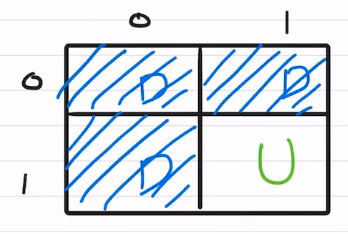
\includegraphics[width=0.3\textwidth]{figs/rectanglelemma-basecase.png}
		\caption{Base Case illustration for rectangle lemma.}
		\label{fig:rectanglelemma-basecase}
	\end{figure}
	
	Induction Step. Suppose the statement is true for $n - 1$. Then, we have a $n \times n$ rectangle that can be split into four quadrants, according to their first coordinate. See Figure \ref{fig:rectanglelemma-is} for an illustration. The inner blue-ish part is the original rectangle. Notice that breaking a rectangle into quadrants by fixing one coordinate results in four rectangles.
	
	Call $b_{-1} = (b_2, \dots, b_n)$ and $a_{-1} = (a_2, \dots, a_n)$. Then define
	\begin{equation}
		R_{-1} = \left\{ 
			(a_{-1}, b_{-1}) : ((0, a_{-1}), (0, b_{-1})) \in R \quad OR \quad ((0, a_{-1}), (1, b_{-1})) \in R
		\right\}
	\end{equation}
	similarly for columns 
	\begin{equation}
		C_{-1} = \left\{ 
			(a_{-1}, b_{-1}) : ((0, a_{-1}), (0, b_{-1})) \in R \quad OR \quad ((1, a_{-1}), (0 , b_{-1})) \in R
		\right\}
	\end{equation}
	
	Then, we immediately know 
	\begin{equation}
		R_{-1} \cap U_{n-1} = \emptyset
	\end{equation}
	which must be true since $R \cap U = \emptyset$. This implies, by induction, that
	\begin{equation}
		|R_{-1} \cap D_{n - 1}| \leq 2^{n - 1}
	\end{equation}
	
	For column, similarly, 
	\begin{equation}
		C_{-1} \cap U_{n - 1} = \emptyset \quad \overset{(induction)}{\implies} \quad |C_{-1} \cap D_{n-1} | \leq 2^{n-1}
	\end{equation}
	
	Ideally, $|R \cap D| \leq |R_{-1} \cap D_{n - 1} | + |C_{-1} \cap D_{n - 1}|$. To show this, we need to rule out the case where we select something in all of the quadrant except for the bottom right one. Imagine we have 
	\begin{equation}
		\begin{cases}
			((0, a_{-1}), (0, b_{-1})) \in R \\
			((1, a_{-1}), (0, b_{-1})) \in R \\
			((0, a_{-1}), (1, b_{-1})) \in R
		\end{cases}
	\end{equation}
	but then this would imply $((1, a_{-1}), (1, b_{-1})) \in R$ because of exchange property, which implies $R\cap U \neq \emptyset$ which results in a contradiction. So it must be the case that $|R \cap D| \leq |R_{-1} \cap D_{n - 1} | + |C_{-1} \cap D_{n - 1}|$. This completes the proof. \qed
	
	\begin{figure}
		\center 
		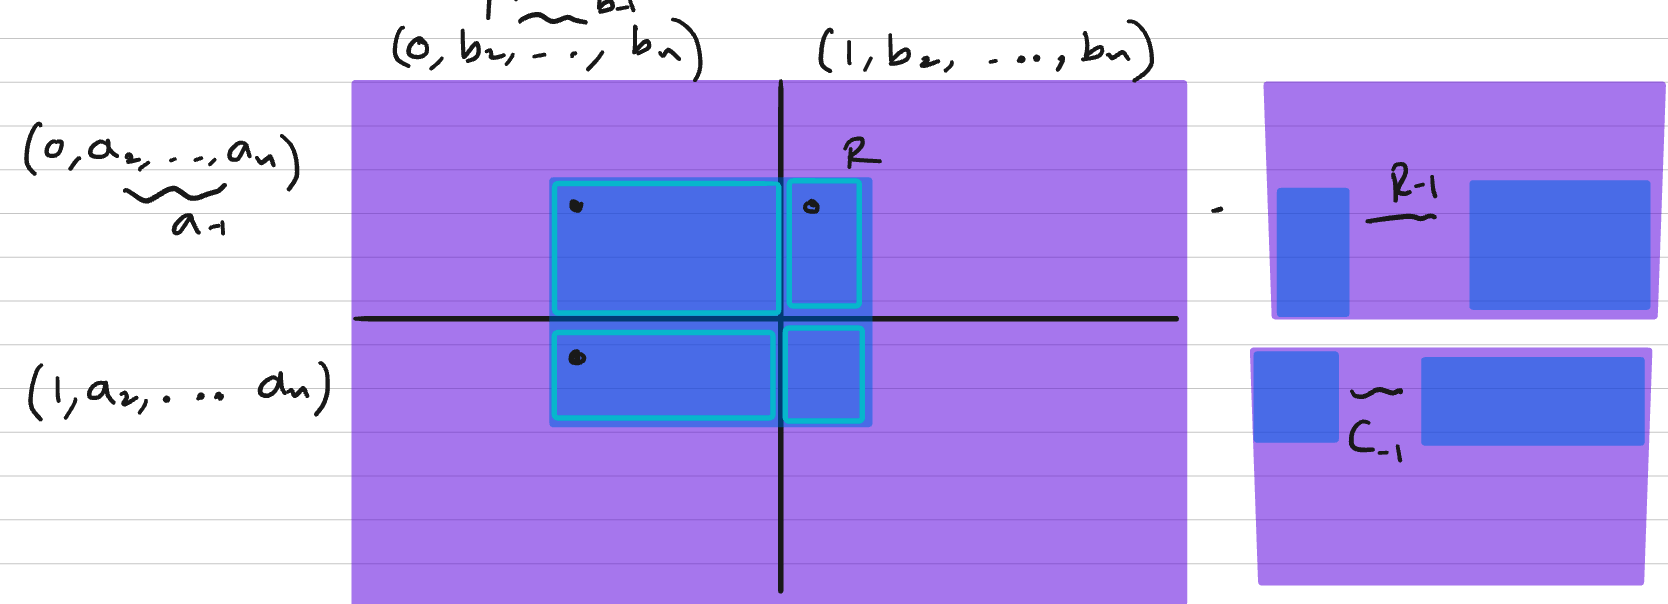
\includegraphics[width=0.9\textwidth]{figs/rectanglelemma-is.png}
		\caption{Inductive step illustration for rectangle lemma.}
		\label{fig:rectanglelemma-is}
	\end{figure}
\end{proof}

\paragraph{Proof Structure Look Back} 
\begin{equation}
	\begin{matrix}
		nnr(M_n) \geq (3/2)^n \\
		\downdownarrows \quad (FMPTW12) \\
		nnr(PartialSlack(CP_n)) \geq (3/2)^n \\
		\downdownarrows \quad (Y88) \\
		nnr(Slack(CP_n)) \geq (3/2)^n \\
		\downdownarrows \quad (Y88) \\
		XC(CP_n) \geq (3/2)^n
	\end{matrix}
\end{equation}
In a chain
\begin{align}
	(3/2)^n 
	&\leq nnr(M_n) \\
	&= nnr(PartialSlack(CP_n)) \\
	&\leq nnr(Slack(CP_n)) \\
	&\leq XC(CP_n)
\end{align}
where the step $nnr(Slack(CP_n))$ involves a brilliant application of Farkas' Theorem. 



